\chapter{Funktionen}

\section{Eigene Funktionen  definieren}

In den vergangenen Lektionen haben Sie bereits viele Funktionen (=Befehle) verwendet, wie beispielsweise \lstinline|t.forward(100)| oder \lstinline|print()|. Im Allgemeinen erkenenn Sie Befehle daran, dass Sie ein mit einem \textbf{Wort} beginnen, wie beispielsweise \lstinline|t.forward| oder \lstinline|print|, auf welches Klammern sowie ein oder mehrere Werte folgen. Diese Werte werden \textbf{Parameter} genannt und dienen dazu, das Verhalten einer Funktion leicht abzuändern, so dass beispielsweise in der Funktion \lstinline|t.fd()| 50 oder 100 Pixel gezeichnet werden. Um unseren Code leserlicher und kürzer zu machen, können wir auch eigene Definitionen schreiben!

\begin{myexample}
Wir betrachten nochmals den Code aus \cref{myexample:blume}:

\lstinputlisting[language=Python,caption=\texttt{blume.py},label=listing:blume]{GrundlagenInfo/00_Programmieren/Skript/Code/K01_Intro/blume.py}

Wir könnten den Code leserlicher machen, indem wir einen Befehl für eine Quadrat und einen Befehl für das gesamte Muster erstellen:

\begin{lstlisting}[escapechar=!]
import turtle as t

def !\colorbox{HotPink}{viereck()}!: !\tikzmark{to2ex}!
    repeat 4:
        fd(100)
        rt(360/4)

def !\colorbox{CornflowerBlue}{viereck\_blume()}!:!\tikzmark{to1ex}! 
    repeat 10:
        !\colorbox{HotPink}{viereck()}! !\tikzmark{from2ex}!
        rt(360/10)

!\colorbox{CornflowerBlue}{viereck\_blume()}! !\tikzmark{from1ex}!

t.done()
\end{lstlisting}
\begin{tikzpicture}[overlay,remember picture]
\draw[red,-stealth] (from1ex.north) to[bend right] node[fill=CornflowerBlue,rounded corners,font=\sffamily\small,text=white] {\emoji{cook} Aufruf} (to1ex);
\draw[red,-stealth] (from2ex.north) to[bend right]
node[fill=CornflowerBlue,rounded corners,font=\sffamily\small,text=white] {\emoji{cook} Aufruf} (to2ex);
\end{tikzpicture}

Eine Funktion beginnt immer mit dem Wort \lstinline|def|, gefolgt von einem Namen sowie Klammern. Innerhalb des eingerückten Bereichs wird eine Aktivität beschrieben. Die Aktivität wird aber erst ausgeführt, sobald der Code aufgeruft wird!

Im übertragenen Sinne kann man sich Definitionen vorstellen wie Kochrezepte, die eine Ablauf beschreiben. Die Funktion beschreibt dabei ein Programmablauf, also ein ``Rezept'', ausgeführt (``gekocht'') wird dieses jedoch erst, sobald das Programm abgerufen wird (auf Zeile 13 und 10 im obigen Beispiel).

Das Schreiben von Definitionen hat mehrere Vorteile:
\begin{itemize}
\item Der Code wird \textbf{modular}: Man kann nun einfachere Funktionen schreiben, wie beispielsweise \lstinline|viereck()|, und komplexere Funktionen, die Unter-Funktionen aufrufen, wie beispielsweise \lstinline|viereck_blume()|.
\item Der Code wird \textbf{übersichtlicher}: jeder Teil-Aktivität ist eine Funktion!
\item Falls das komplexere Programm nicht das gewünschte Resultat liefert, können wir es \textit{debuggen}, indem wir die einfacheren Funktionen zuerst aufrufen und sicherstellen, dass diese richtig funktionieren.
\end{itemize}

Dass der ursprüngliche Code nun übersichtlicher ist, wird in folgenden zwei Code-Varianten ersichtlich:

\begin{center}
\begin{minipage}{.4\textwidth}
\begin{lstlisting}[escapechar=!]
import turtle as t

for _ in range(10):    !\tikzmark{repOuterStart}!
    for _ in range(4):!\tikzmark{repInnerStart}!
        t.fd(100)
        t.rt(360 / 4)      !\tikzmark{repInnerEnd}!
    t.fd(360 / 10)         !\tikzmark{repOuterEnd}!
    
t.done()
\end{lstlisting}
\end{minipage}\hfill\begin{minipage}{.4\textwidth}
\begin{lstlisting}[escapechar=!]
import turtle as t

!\tikzmark{repInnerStartTo}!def viereck():
    for _ in range(4):
        t.fd(100)
!\tikzmark{repInnerEndTo}!        t.rt(360 / 4)

!\tikzmark{repOuterStartTo}!def viereck_blume():
    for _ in range(10):
        viereck()
!\tikzmark{repOuterEndTo}!        t.rt(360/10)

quadrat_blume()

t.done()
\end{lstlisting}
\end{minipage}
\end{center}
\begin{tikzpicture}[overlay, remember picture,
    every edge/.append style = { ->, thick, >=stealth, red!70},
    every node/.style={draw=red!50,fill=red!50!white,text=black,rounded corners}]
	\drawBrace{0em}{repInnerStart}{repInnerEnd}{}{.5}{};
		\drawBrace{-.5em}{repInnerStartTo}{repInnerEndTo}{}{.5}{mirror};
		% arrow pointing from one code to other
		\draw[->, style={thick, >=stealth, red!70}] (repInnerStartrepInnerEnd-coord-arrow) to (repInnerStartTorepInnerEndTo-coord-arrow);
		\drawBrace{1em}{repOuterStart}{repOuterEnd}{}{.75}{};
			\drawBrace{-.5em}{repOuterStartTo}{repOuterEndTo}{}{.25}{mirror};
			% arrow pointing from one code to other
			\draw[->, style={thick, >=stealth, red!70}] (repOuterStartrepOuterEnd-coord-arrow) to (repOuterStartTorepOuterEndTo-coord-arrow);
\end{tikzpicture}

Wichtig zu beachten für die Übersichtlichkeit des Codes sind folgende Aspekte:
\begin{itemize}
\item Innere Schleifen sollten wenn immer möglich vermieden und durch Definitionen ersetzt werden
\item Definitions-Namen sollten möglichst selbsterklärend und ``sprechend'' sein, sie sollten also klar beschreiben, was die Aktivität tut! %TODO Beispiel
\end{itemize}
\end{myexample}

\begin{myexercise}
Führen Sie folgend Code zuerst aus und betrachten Sie das Resultat. Schreiben Sie Code um, indem Sie zwei Funktionen schreiben: \lstinline|viertelkreis()| und 
\lstinline|abgerundetes_quadrat()|.

\begin{lstlisting}
import turtle as t

for _ in range(4):
    for _ in range(9):
        t.fd(4)
        t.lt(10)
    t.fd(100)
\end{lstlisting}

\begin{myanswer}
\begin{center}
\begin{minipage}{.4\textwidth}
\begin{lstlisting}[escapechar=!]
import turtle as t

for _ in range(4):    !\tikzmark{repOuterStart}!
    for _ in range(9):!\tikzmark{repInnerStart}!
        t.fd(4)
        t.lt(10)      !\tikzmark{repInnerEnd}!
    t.fd(100)         !\tikzmark{repOuterEnd}!
\end{lstlisting}
\end{minipage}\hfill\begin{minipage}{.4\textwidth}
\begin{lstlisting}[escapechar=!]
import turtle as t

!\tikzmark{repInnerStartTo}!def viertelkreis():
    for _ in range(9):
        t.fd(4)
!\tikzmark{repInnerEndTo}!        t.lt(10)

!\tikzmark{repOuterStartTo}!def abgerundetes_quadrat():
    for _ in range(4):
        viertelkreis()
!\tikzmark{repOuterEndTo}!        t.fd(100)

abgerundetes_quadrat()
\end{lstlisting}
\end{minipage}
\end{center}
\begin{tikzpicture}[overlay, remember picture,
    every edge/.append style = { ->, thick, >=stealth, red!70},
    every node/.style={draw=red!50,fill=red!50!white,text=black,rounded corners}]
	\drawBrace{0em}{repInnerStart}{repInnerEnd}{}{.5}{};
		\drawBrace{-.5em}{repInnerStartTo}{repInnerEndTo}{}{.5}{mirror};
		% arrow pointing from one code to other
		\draw[->, style={thick, >=stealth, red!70}] (repInnerStartrepInnerEnd-coord-arrow) to (repInnerStartTorepInnerEndTo-coord-arrow);
		\drawBrace{1em}{repOuterStart}{repOuterEnd}{}{.75}{};
			\drawBrace{-.5em}{repOuterStartTo}{repOuterEndTo}{}{.25}{mirror};
			% arrow pointing from one code to other
			\draw[->, style={thick, >=stealth, red!70}] (repOuterStartrepOuterEnd-coord-arrow) to (repOuterStartTorepOuterEndTo-coord-arrow);
\end{tikzpicture}
\end{myanswer}
\end{myexercise}

\begin{myexercise}
Packen Sie Ihre Lösung aus \cref{myexercise:Haus} in eine Funktion mit dem Namen \lstinline|def haus()|. Testen Sie zunächst, ob die  Funktion wirklich das gewünschte Resultat liefert (ein einzelnes Haus) indem Sie die Funktion aufrufen. Schreiben Sie dann eine zweite Funktion \lstinline|def haeuserreihe():|, welche eine Häuserreihe aus 5 Häusern zeichnet, indem \lstinline|haus()| fünfmal aufgerufen wird.
\end{myexercise}




% TODO weitere Übungen
\section{Parameter}

\begin{myexample}\label{example:params}
Stellen Sie sich vor, sie wollen drei unterschiedlich grosse Quadrate zeichnen. Sie könnten folgendermassen vorgehen:

\lstinputlisting[language=Python,caption=\texttt{noparams.py},label=listing:blume]{GrundlagenInfo/00_Programmieren/Skript/Code/K03_Functions/squares_noparams.py}

Das ging gerade noch! Was jedoch, wenn Sie 20 unterschiedlich grosse Quadrate zeichnen wollen? Brauchen Sie dann 20 Definitionen? Zum Glück nicht, da Sie hierfür Parameter verwenden können, wie in folgendem Beispiel gezeigt:

\lstinputlisting[language=Python,caption=\texttt{params.py},label=listing:blume]{GrundlagenInfo/00_Programmieren/Skript/Code/K03_Functions/squares_params.py}

\begin{lstlisting}[escapechar=!]
import turtle as t

def quadrat(!\colorbox{DeepPink}{la\tikzmark{arrowTo1}enge}!):
	repeat 4:
		t.fd(!\colorbox{DeepPink}{la\tikzmark{arrowTo2}enge}!) 
		t.rt(90)

quadrat(!\colorbox{DeepPink}{5\tikzmark{arrow1From}0}!)
quadrat(!\colorbox{DeepPink}{1\tikzmark{arrow2From}00}!)
quadrat(!\colorbox{DeepPink}{1\tikzmark{arrow3From}50}!)
\end{lstlisting}
\begin{tikzpicture}[overlay,remember picture]
    \draw[red,-stealth] (arrow1From.north) to[bend right] node[right, yshift=-.8cm, fill=RoyalBlue,text=white,rounded corners] {\emoji{handshake} Übergabe} (arrowTo1);
    \draw[red,-stealth] (arrowTo1.south) to[bend right] (arrowTo2);
    \draw[red,-stealth] (arrow2From.south) to[bend right] (arrowTo1);
    \draw[red,-stealth] (arrow3From.south) to[bend right] (arrowTo1);
\end{tikzpicture}
\end{myexample}

\begin{myexercise}
Schreiben Sie folgende Funktionen und testen Sie diese, indem Sie sie auf Moodle hochladen:

\begin{itemize}
\item \lstinline|def summiere(x1, x2)|: Berechnet die Summe zweier Parameter \lstinline|x1| und \lstinline|x2| und gibt das Resultat auf der Konsole aus.
\item \lstinline|def summe_quadrate(x1, x2)|: Berechnet die Summe von \texttt{x1}$^2$ + \texttt{x2}$^2$ und gibt das Resultat auf der Konsole aus.
\item \lstinline|def pizzaparty(personen, stuecke)|: Berechnet die Anzahl Pizza-Stücke, die bei \texttt{personen} Personen übrigbleiben, aus \cref{ex:modulo-pizza} und gibt sie per \lstinline|print| aus.
\end{itemize}
% TODO implement on Moodle
\end{myexercise}

\subsection{Lebensdauer (\textit{scope}) einer Variable}

Im Code aus \cref{example:params} wird bei \textit{jedem Aufruf} der Definition \lstinline|quadrat| eine neue Variable \texttt{laenge} erstellt, welche nur \textit{innerhalb} der Funktion existiert und welche jedes Mal einen anderen Wert hat. Den Wert erhält die Variable zum Zeitpunkt des \textit{Aufrufs} der Funktion, also auf den Zeilen 8, 9 und 10!

Die Variable \texttt{laenge} existiert also nur innerhalb der Definition \lstinline|quadrat| Wenn wir nach Zeile 6 im Hauptprogramm (nicht eingerückt) den Befehl \texttt{print(laenge)} eingeben würden, würden wir eine Fehlermeldung erhalten, da es die Variable nicht mehr gibt. Parameter sind also immer \textbf{\textit{lokale} Variablen}, ebenso wie Variablen, welche wir innerhalb von Funktion erstellen. Diese Variablen \enquote{sterben} nach Ausführung der Definition, daher spricht man auch von der Lebensdauer einer Variable, bzw. von deren Reichweite (en. \textit{scope})

Variablen, welche im Hauptprogramm (nicht eingerückt) erstellt werden, sind sogenannte \textbf{\textit{globale} Variablen}.

\begin{myexercise}\label{ex:local-global}
Beschreiben Sie, welche der Variablen im unten stehenden Code lokal oder global sind, und welche Variablen auch Parameter sind. Sie sollten insgesamt 5 Variablen finden!
\lstinputlisting[language=Python,caption=\texttt{houses.py},label=listing:blume]{GrundlagenInfo/00_Programmieren/Skript/Code/K03_Functions/houses.py}

\begin{myanswer}
\begin{enumerate}
\item \lstinline|laenge|: lokale Variable, Parameter der Funktion \lstinline|haus()|
\item \lstinline|anzahl_mauern|: lokale Variable
\item \lstinline|laenge_pro_haus|: lokale Variable, Parameter der Funktion \lstinline|haeuserreihe()|
\item \lstinline|anzahl_haeuser|: lokale Variable
\item \lstinline|seitenlaenge|: globale Variable
\end{enumerate}
\end{myanswer}
\end{myexercise}

\begin{myexercise}
Was könnte der Vorteil von \textit{lokalen Variablen} sein?
\begin{myanswer}
Falls Sie mehrere Funktionen schreiben, können Sie dieselben Variabelnamen und Parameter-Namen innerhalb der Funktionen verwenden, da diese nichts miteinander zu tun haben. Im Code aus \cref{ex:local-global} hätten wir auch in beiden Funktionen \texttt{laenge} schreiben können.
\end{myanswer}
\end{myexercise}

\subsection{Mehrere Parameter}
Man kann beliebig viele Parameter verwenden in Funktionen. Wichtig dabei ist, diese je durch ein Komma zu trennen.

\begin{myexample}\label{ex:multiple-params}
In folgendem Beispiel kann nicht nur die Anzahl Ecken, sondern auch die Farbe eines Polygons übergeben werden.
\lstinputlisting[language=Python,caption=\texttt{farb\_vieleck.py},label=listing:blume]{GrundlagenInfo/00_Programmieren/Skript/Code/K03_Functions/farb_vieleck.py}
\begin{figure}[H]
\centering
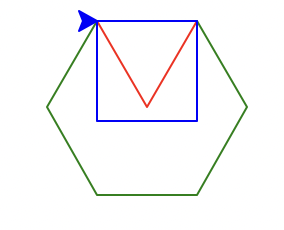
\includegraphics[width=0.2\linewidth]{GrundlagenInfo/00_Programmieren/Figures/mehrere-parameter}
\end{figure}
\end{myexample}

\begin{myexercise}
Ändern Sie den Code aus \cref{ex:multiple-params} so ab, dass zusätzlich auch noch die Stiftdicke verändert werden kann. Verwenden Sie dazu einen weiteren Parameter sowie den Befehl \texttt{t.width(...)}.
\end{myexercise} 

\section{Befehle / Funktionen mit Parameter, mit \texorpdfstring{\lstinline|return|}{return}}
\subsection{Einzelne Funktionen}

Wie Sie bereits wissen, können Definitionen mit Kochrezepten verglichen werden: Sie beschreiben einen Ablauf, ohne jedoch diesen auszuführen. Damit der Ablauf ausgeführt wird, müssen Sie die Definition aufrufen. Dies kann nützlich sein, wenn sie eine Aufgabe mehrmals und in unterschiedlichen Varianten ausführen wollen, wie beispielsweise das Zeichnen einer Spirale. Eine wichtige Limitation von Definitionen war bisher, dass Sie zwar Dinge berechnen, jedoch keine Werte an das Hauptprogramm zurückgeben konnten. In diesem Kapitel lernen wir, wie Funktionen wie ``Sous-Chefs'' in einer komplexen Küche Zutaten (Parameter) entgegennehmen und Resultate an andere ``Sous-Chefs''  (Definitionen) weitergeben können.


Definitionen können zudem Inputs entgegennehmen, sogenannte \textbf{Parameter}. Wir konnten zwar bisher einen Wert einer Variable mittels \lstinline|print| drucken, Bisher konnten Sie jedoch nichts an das Hauptprogramm zurückgeben. Dies bedeutet, dass alle Variablen, die wir je in einer Definition erstellt haben, nur in dieser Definition ``lebten'' und nicht mehr zugreifbar waren, nachdem das Programm beendet wurde.

\begin{myexample}\label{ex:sum-noreturn}
Betrachten Sie folgenden Code. Weshalb führt er zu einer Fehlermeldung?
\begin{lstlisting}
def summiere(x1, x2):
    summe = x1 + x2
    
summiere(3, 5)
print(summe)
\end{lstlisting}
Die Konsole gibt folgende Meldung aus: \texttt{[Zeile: 5] NameError: name 'summe' is not defined}. Dies bedeutet, dass die Variable \lstinline|summe| auf Zeile 5 nicht existiert. Die Fehlermeldung erklärt sich dadurch, dass alle Variablen, die innerhalb einer Definition erstellt werden, nur innerhalb dieser Definition ``\textit{leben}'', also existieren. Dass Variablen mittels dem Befehl \lstinline|return| auch an das Hauptprogramm ``zurückgegeben'' werden können, lernen wir in diesem Kapitel.
\end{myexample}

Eine Funktion kann man sich vorstellen wie ein Kochrezept, das einige Zutaten entgegennimmt und ein Resultat (Gericht) zurückgibt. Die Zutaten, oder ``Inputs'', werden dabei häufig als ``\textbf{Parameter}'' bezeichnet, währenddem das fertige Gericht, oder ``Resultat'' häufig als ``\textbf{\lstinline|return|-Wert}'' bezeichnet wird. Diese Idee ist in \cref{fig:funktion-einzeln}) veranschaulicht.

\begin{figure}[H]
% Use the \drawCube macro to draw various cubes
\centering
\begin{tikzpicture}
\drawCube{1}{0}{2}{3}
\node[fill=blue!50, rounded corners] (input1) at (llD11val){3};
\node[fill=blue!50, rounded corners] (input2) at (llD21val){12};
\draw[thick,->] (input1) -- (in11);
\draw[thick,->] (input2) -- (in12);
\node[fill=green!50, rounded corners](outVal1) at (5,-.6,3){36};
\draw[thick,->] (out1) -- (outVal1);
\end{tikzpicture}
\caption{Illustration einer Funktion mit Inputs (Parametern) und Outputs (\lstinline|return|-Wert)}
\label{fig:funktion-einzeln}
\end{figure}

\begin{myexample}
Betrachten Sie nochmals den folgenden, leicht modifizierten Code aus \cref{ex:sum-noreturn}. Wenn wir den Wert mit \lstinline|return| an das Hauptprogramm zurückgeben und in einer Variable (im Hauptprogramm, auf Zeile 5) abspeichern, funktioniert der Code nun.\\

\begin{minipage}{\linewidth}
\begin{lstlisting}
def summiere(x1, x2):
    summe = x1 + x2
    return (*@\colorbox{RoyalBlue!50}{sum\tikzmark{arrowFromEx01}me}@*)
    


(*@\colorbox{ForestGreen!50}{re\tikzmark{arrowToEx02}s}@*)=(*@\colorbox{RoyalBlue!50}{summie\tikzmark{arrowToEx01}re(3, 5)}@*)
print(res)
\end{lstlisting}
\begin{tikzpicture}[overlay,remember picture]
   % Wert zurückgeben
	\draw[RoyalBlue,-stealth, thick] (arrowFromEx01.south) to[bend left] node[align=left, pos=.15, right, fill=RoyalBlue,fill opacity=.5, text opacity=1, text=black,rounded corners] {Wert an das Hauptprogramm zurückgeben...} (arrowToEx01.north);
	
	\draw[ForestGreen,-stealth, thick] (arrowToEx01.north) to[bend right] node[align=left, pos=.7, above right, fill=ForestGreen,fill opacity=.5, text opacity=1, text=black,rounded corners] {...\textit{und} Wert in Variable speichern, z.B. \lstinline|res|} (arrowToEx02.north);
\end{tikzpicture}
\end{minipage}
\end{myexample}

\begin{mysubmission}
Geben seien die Höhe \texttt{h} und die Grundseite \texttt{b} eines Dreiecks. Schreiben Sie eine Funktion \lstinline|def flaeche_dreieck(h, b)|, welche den Flächeninhalt dieses Dreiecks berechnet und mit \lstinline|return| zurückgibt.

Überprüfen Sie die Korrektheit Ihrer Funktion, indem Sie sie auf Moodle hochladen.
\begin{myanswer}
\begin{lstlisting}
def flaeche_dreieck(h, b):
    return h*b/2
\end{lstlisting}
\end{myanswer}
\end{mysubmission}

\begin{mysubmission}
Geben sei eine ganze Zahl \texttt{n}. Schreiben Sie eine Funktion \lstinline|def square(n)|, welche das Quadrat von \lstinline|n| berechnet und mit \lstinline|return| zurückgibt.

Überprüfen Sie die Korrektheit Ihrer Funktion, indem Sie sie auf Moodle hochladen.
\begin{myanswer}
\begin{lstlisting}
def square(n):
    return n*n
\end{lstlisting}
\end{myanswer}
\end{mysubmission}



\subsection{Mehrere Funktionen}
Wozu kann ein \lstinline|return| eigentlich nützlich sein? Wenn Sie Code schreiben, wird dieser oftmals schnell komplizierter. Somit kann es hilfreich sein, die einzelnen Schritte in Unter-Programme aufzuteilen. Dies erleichtert zudem die \textbf{Modularisierung} und \textbf{Wiederverwendbarkeit} von Code: Beispielsweise könnte eine Funktion, die das Maximum einer Liste berechnet, an verschiedenen Orten in einem längeren Programm mehrmals zum Einsatz kommen

Zum Vergleich: stellen Sie sich vor, Sie arbeiten in einer edlen Michelin-Sterne-Küche an einem raffinierten Gericht, in das viele Arbeitsschritte involviert sind. Häufig müssen in solchen Restaurants bis zu 200 Schritte pro Gericht ausgeführt werden. Daher könnte es sinnvoll sein, einzelne Aufgaben, wie beispielsweise die Herstellung der Saucen, an Ihre Sous-Chefs zu delegieren, und eine Person zu bestimmen, die das ganze Gericht zusammenfügt. Häufig werden Funktionen genau mit solchen komplexen Aufgaben im Hinterkopf geschrieben. Diese Idee ist in \cref{fig:funktionen-mehrere} illustriert.

\begin{figure}[H]
% Use the \drawCube macro to draw various cubes
\centering
\begin{tikzpicture}
\drawCube{1}{0}{2}{3}
% feed input values into a1
\node[fill=blue!50, rounded corners] (input1) at (llD11val){3};
\node[fill=blue!50, rounded corners] (input2) at (llD21val){12};
\draw[thick,->] (input1) -- (in11);
\draw[thick,->] (input2) -- (in12);
\node[fill=green!50, rounded corners](outVal1) at (5,-.6,3){36};
\draw[thick,->] (out1) -- (outVal1);
\drawCube{2}{5.25}{3}{3}
\drawCube{3}{10.5}{2}{3}
\draw[thick,->,rounded corners] (out1) -- ++(0,-3.25,0) -- ++(3.15,0,0)node[below]{\lstinline[language=Python,style=TigerJython,basicstyle=\ttfamily]{return out1}} -- ++(4.65,0,0) -- (in31);
\end{tikzpicture}
\caption{Illustration einer Code-Struktur, bei welcher mehrere Funktionen zusammenarbeiten}
\label{fig:funktionen-mehrere}
\end{figure}

In \cref{fig:funktionen-mehrere} haben wir eine Funktion \lstinline|a1|, die zwei Parameter entgegennimmt (\lstinline|x1| und \lstinline|x2|). Mit diesen Parametern macht sie etwas (z.B. die Summe berechnen, ein Quadrat zeichnen oder irgend eine sonstige Aufgabe) und gibt danach einen neuen, berechneten Wert \lstinline|a1| zurück. Dieser kann im Hauptprogramm abgespeichert und an andere Funktionen weitergegeben werden, beispielsweise an die Funktion \lstinline|a3|.

\begin{myexample}
Stellen Sie sich vor, Sie arbeiten für einen Supermarkt und sollten den Preis Ihrer Produkte berechnen. Sie kaufen Ihre Artikel bei einem Grossverteiler ein, daher erhalten Sie auf alle Produkte 10\% Rabatt. Der Grossverteiler befindet sich im Ausland, Sie müssen also noch 7\% Mehrwertsteuer hinzufügen. Der Grossverteiler gibt Ihnen den Original-Preis Ihrer Waren \textit{vor} Rabatt und \textit{vor} Mehrwertsteuer.

Folgender Code berechnet den Endpreis, für den Sie ihre Waren verkaufen werden, indem folgende zwei Funktionen aufgerufen werden:
\begin{enumerate}
\item \lstinline|berechne_rabatt| berechnet den Preis nach Abzug eines Rabatts für ein Produkt.
\item \lstinline|berechnet_gesamtpreis| ruft \lstinline|berechne_rabatt| auf und fügt zum rabattierten Preis die Mehrwertsteuer hinzu.
\end{enumerate}

\begin{minipage}{\linewidth}
\begin{lstlisting}
def berechne_rabatt(preis, rabatt_prozent):
    rabatt = preis * (rabatt_prozent / 100)
    (*@\colorbox{CornflowerBlue}{return preis - \tikzmark{arrowFromEx11} rabatt}@*) # Gibt den Preis nach Abzug des Rabatts zurück


def berechne_gesamtpreis(preis, rabatt_prozent, mehrwertsteuer_prozent):
    (*@\colorbox{CornflowerBlue}{rabatt\tikzmark{arrowToEx11}preis}@*) = berechne_rabatt(preis, rabatt_prozent)
    mwst = rabattpreis * (mehrwertsteuer_prozent / 100)
    return (*@\colorbox{CornflowerBlue}{rabattpre\tikzmark{arrowFromEx12}is + mwst}@*)  # Gibt den Gesamtpreis inklusive Mwst. zurück


# Anwendung
preis = 100  # Basispreis in CHF
rabatt_prozent = 10  # Rabatt in %
mehrwertsteuer_prozent = 7.7  # Mehrwertsteuer in %

(*@\colorbox{CornflowerBlue}{endp\tikzmark{arrowToEx12}reis}@*) = berechne_gesamtpreis(preis, rabatt_prozent, mehrwertsteuer_prozent)
print("Der Endpreis nach Rabatt und Mehrwertsteuer ist:", endpreis)
\end{lstlisting}
\begin{tikzpicture}[overlay,remember picture]
   % Wert zurückgeben
	\draw[red,-stealth] (arrowFromEx11.north) to[bend left] node[pos=.3, right, fill=RoyalBlue,fill opacity=.5, text opacity=1, text=black,rounded corners] {Wert zurückgeben (und speichern)} (arrowToEx11);
	\draw[red,-stealth] (arrowFromEx12.north) to[bend left] node[pos=.2, right, fill=RoyalBlue, fill opacity=.5, text opacity=1, text=black,rounded corners] {Wert zurückgeben  (und speichern)} (arrowToEx12);
\end{tikzpicture}
\end{minipage}
\end{myexample}



\begin{myexample}
Mit folgendem Code können wir die Turtle eine Spirale aus mehreren Kreisen zeichnen lassen:\\
\begin{minipage}{.65\textwidth}
\begin{lstlisting}
from gturtle import *
makeTurtle()
hideTurtle()

def vieleck(umfang, ecken):
    repeat ecken:
        fd(umfang/ecken)
        rt(360/ecken)

def vieleck_muster(umfang, ecken):
    while umfang>50:
        vieleck(umfang, ecken)
        umfang-=10
        rt(10)
    
vieleck_muster(500,35)
\end{lstlisting}

\end{minipage}
\begin{minipage}{.25\textwidth}
\begin{figure}[H]
	\centering
    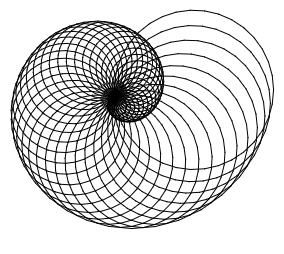
\includegraphics[keepaspectratio, width=\textwidth]{GrundlagenInfo/00_Programmieren/Figures/spirale.png}
\end{figure}
\end{minipage}\\

Leider ist unsere Turtle etwas müde und sollte nicht zu viel laufen. Daher möchten wir fortlaufend die Gesamtdistanz berechnen, um am Ende herauszufinden, ob unsere Turtle zu viel Strecke zurückgelegt hat. Dies können wir tun, indem wir die Funktion einen Wert zurückgeben lassen:
\begin{lstlisting}
from gturtle import *
makeTurtle()
hideTurtle()

def vieleck(umfang, ecken):
    repeat ecken:
        fd(umfang/ecken)
        rt(360/ecken)

def vieleck_muster(umfang, ecken):
	(*@\colorbox{CornflowerBlue}{gesamtdistanz=0}@*)
    while umfang>50:
        vieleck(umfang, ecken)
        (*@\colorbox{CornflowerBlue}{gesamtdistanz+=umfang}@*)
        umfang-=10
        rt(10)
    (*@\colorbox{CornflowerBlue}{return gesamtdistanz}@*)
    
(*@\colorbox{CornflowerBlue}{gesamtdistanz = }@*)vieleck_muster(500,35)
(*@\colorbox{CornflowerBlue}{print(gesamtdistanz)}@*)
\end{lstlisting}


\end{myexample}


\begin{myexercise}
Schreiben Sie eine Python-Funktion \lstinline|def notenskala(maxPunkte, erreichtePunkte)|, welche die erreichte Note in Abhängigkeit der maximal möglichen Punktzahl und der erreichten Punktzahl berechnet und per \lstinline|return| zurückgibt. Verwenden Sie dafür die folgende Formel:

\[ \text{note} = \frac{\text{erreichtePunkte}}{\text{maxPunkte} }\cdot 5 + 1 \]
\begin{myanswer}
\begin{lstlisting}
def notenskala(maxPunkte, erreichtePunkte):
    return erreichtePunkte/maxPunkte * 5 + 1
\end{lstlisting}
\end{myanswer}
\end{myexercise}



\subsection{Weitere Übungen}

\begin{mychallenge}[\emoji{robot} \textbf{R2-D2}]

Der Mikrocontroller einer R2-D2 Roboter-Einheit wurde beschädigt. Der Roboter kann deshalb nur noch einzelne, geradlinige \enquote{Schritte} nach links (l), rechts (r), oben (o) oder unten (u) (um jeweils eine Längeneinheit) durchführen. Die Bewegungsanweisung erhält der Roboter in Form des Strings \tjinline{bewegung}. Der String \tjinline{bewegung = 'lollru'} würde zum Beispiel dem Bewegungsablauf links, oben, links, links, rechts und unten (um jeweils eine Längeneinheit) entsprechen. Die R2-D2-Einheit bewegt sich auf dem zweidimensionalen Koordinatensystem und startet im Ursprung $(0,0)$.


Schreiben Sie eine Python-Funktion \tjinline{def r2d2(bewegung)}, welche für eine gegebene beliebige Be\-we\-gungs\-an\-wei\-sung \tjinline{bewegung} entscheidet, ob sich der Roboter nach den Bewegungen wieder im Ursprung befindet (\tjinline{return True}) oder nicht (\tjinline{return False}). Hinweis: Auf die einzelnen Buchstaben eines Strings kann ebenso zugegriffen werden wie auf Listenelemente. Falls zum Beispiel \tjinline{wort = "Hallo"}, dann ist \tjinline{wort[0] == "H", wort[1], == "a"} und so weiter. Wie auch bei Listen, kann mit dem Befehl \tjinline{len(wort)} die Länge (Anzahl Buchstaben) eines Worts bestimmt werden.

\begin{lstlisting}[numbers=none,framexleftmargin=0em,xleftmargin=0em]
Beispiel 1:
Input: bewegung = 'uurol'
Output: False

Beispiel 2:
Input: bewegung = 'rloulr'
Output: True
\end{lstlisting}

\begin{myanswer}
\begin{lstlisting}
def count_symbol(symbol, word):
    count = 0
    for buchstabe in word:
        if buchstabe == symbol:
            count += 1
    return(count)


def r2d2(move):
    l = count_symbol('l', move)
    r = count_symbol('r', move)
    o = count_symbol('o', move)
    u = count_symbol('u', move)
    if (l-r == 0 and o-u == 0):
        return True
    else:
        return False
\end{lstlisting}
\end{myanswer}
\end{mychallenge}